\documentclass[screen, compress]{beamer}
\usepackage[T1]{fontenc}
\usepackage[utf8]{inputenc}
\usepackage[english]{babel}
\usepackage{graphicx}
\usepackage{wrapfig}
\usetheme{Warsaw}

\title[TDT4215 project presentation]{TDT4215: Web-intelligence\\Group 1 project presentation}

\author[Group 1]{Group 1\\
Terje Snarby\\
Even Wiik Thomassen\\
Weilin Wang%
}

%Norges teknisk-naturvitenskapelige universitet
\institute[NTNU]{
\includegraphics[width=0.75\textwidth,height=0.22\textheight]{img/ntnu}}
%\institute[NTNU]{
\includegraphics[width=0.75\textwidth,height=0.22\textheight]{img/ntnu-no}}

\date{\today}

% 1. Explain the system architecture and function and role of the components.
% 2. Which components did you make yourself?
% 3. Present and discuss the results of algorithm.
% 4. Discuss (pros and cons) Explain the selected classification algorithm.
% 5. Evaluation of the classifiers.

\begin{document}

\begin{frame}
\titlepage
\end{frame}


%=====================
\section{Introduction}
%=====================

%-------------------------------
\subsection{System architecture}
%-------------------------------
\begin{frame}{System architecture}
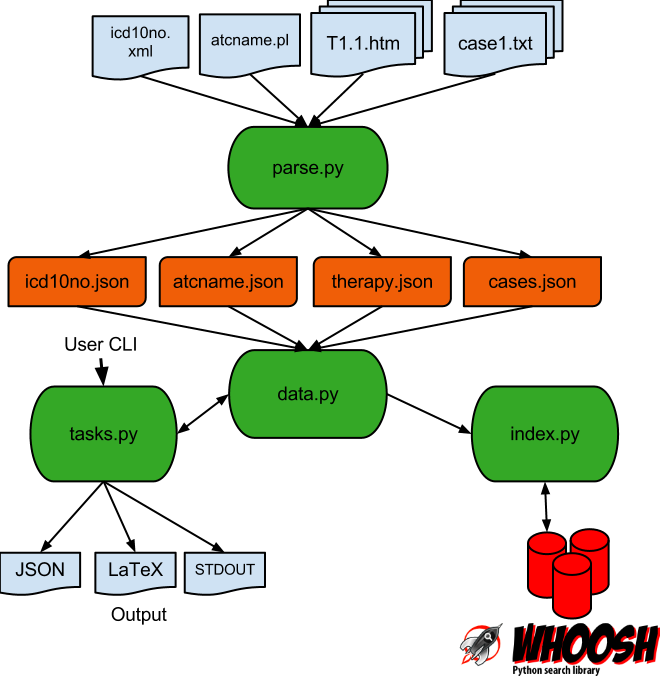
\includegraphics[width=\textwidth,height=0.92\textheight]{img/system_architecture2}
\end{frame}


%============================
\section{Methods and results}
%============================

%------------------------
\subsection{Task 1 and 2}
%------------------------
\begin{frame}{Task 1 and 2 method}
We've used Whoosh + BMF25F something something
\end{frame}

\begin{frame}{Task 1 and 2 results}
\end{frame}

%------------------
\subsection{Task 3}
%------------------
\begin{frame}{Task 3 method}
\end{frame}

\begin{frame}{Task 3 result}
\end{frame}

%------------------
\subsection{Task 4}
%------------------
\begin{frame}{Task 4 method}
\end{frame}

\begin{frame}{Task 4 result}
\end{frame}

%--------------------
\subsection{Task 6 A}
%--------------------
\begin{frame}{Task 6 A method}
\end{frame}

\begin{frame}{Task 6 A result}
\end{frame}

%--------------------
\subsection{Task 6 B}
%--------------------
\begin{frame}{Task 6 B method and result}
\end{frame}


%====================
\section{Evaluations}
%====================
% 4. Discuss (pros and cons) Explain the selected classification algorithm.
% 5. Evaluation of the classifiers.

%------------------------------------
\subsection{Classification algorithm}
%------------------------------------
\begin{frame}{Classification algorithm}
\end{frame}

%------------------------
\subsection{Questions?}
\begin{frame}{Questions?}
%------------------------
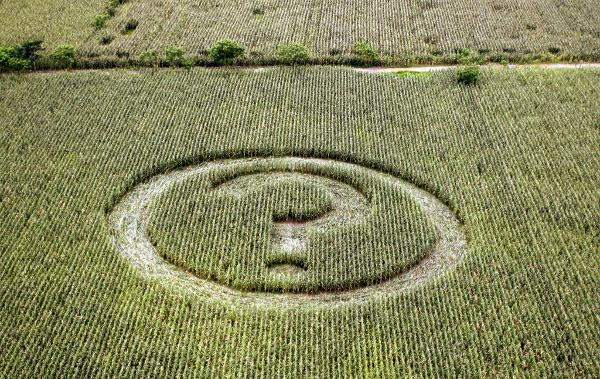
\includegraphics[width=\textwidth]{img/any-questions}
\end{frame}

\end{document}

